\documentclass{beamer}
\usepackage{geometry}
\usepackage[english]{babel}
\usepackage[utf8]{inputenc}
\usepackage{amsmath}
\usepackage{amsfonts}
\usepackage{amssymb}
\usepackage{tikz}
\usetikzlibrary{quotes, angles}
\usepackage{graphicx}
\usepackage{multicol}

%\usepackage{pgfplots}
%\pgfplotsset{width=10cm,compat=1.9}
%\usepackage{pgfplotstable}

\setlength{\headheight}{26pt}%doesn't seem to fix warning

\usepackage{fancyhdr}
\pagestyle{fancy}
\fancyhf{}

%\rhead{\small{13 September 2021}}
\lhead{\small{BECA / Dr. Huson / Geometry Unit 2}}

\renewcommand{\headrulewidth}{0pt}

\title{Mathematics Class Slides}
\subtitle{Bronx Early College Academy}
\author{Christopher J. Huson PhD}
\date{4 October 2021}

\begin{document}
\frame{\titlepage}
\section[Outline]{}
\frame{\tableofcontents}

\section{2.1 Area and volume formulas, 4 October}
\frame
{
  \frametitle{Learning Target: I can calculate area}
  \framesubtitle{7.G.B.6 Solve problems involving area, volume and surface area \hfill \alert{2.1 Monday 4 October}}
  \begin{block}{Do Now: Identify the true statements}
    \begin{multicols}{2}
    \begin{enumerate}
      \item $\angle 1 \cong \angle 2$
      \item $\angle 2 \cong \angle 4$
      \item $m\angle 1 + m\angle 4=180^\circ$
      \item $m\angle 2 + m\angle 3=90^\circ$
  \end{enumerate}
  \begin{center}
  \begin{tikzpicture}[scale=0.5, rotate=15]
    \draw [<->, thick] (0,-1.5)--(10,1.5);
    \draw [<->, thick] (2,3.5)--(7,-3.5);
    \node at (3,.4){1};
    \node at (6,-.6){3};
    \node at (5,1){2};
    \node at (4,-1){4};
  \end{tikzpicture}
  \end{center}
\end{multicols}
\end{block}
  Lesson: Test scoring, mastery; Area formulas \\[0.25cm]
  Homework: Test corrections due Friday
}

\frame
{
  \frametitle{Learning Target:  I can calculate area}
  \framesubtitle{7.G.B.6 Solve problems involving area, volume and surface area}

  \begin{block}{Copy these formulas into your notes}
    
    \begin{enumerate}
    \item Rectangle: $A=l \times w$ (Area equals length times width)
    \item Square: $A=s^2$ (Area equals side length squared)
    \item Triangle: $A=\frac{1}{2} b \times h$ (one half base times height)
    \item Trapezoid: $A=\frac{1}{2} (b_1 +b_2) h$ (Average of bases times height)
    \item Circle: $A=\pi r^2$
    \end{enumerate}
  \end{block}
}

  \frame
  {
    \frametitle{Casio fx-9750GII calculator - due Friday 1 October}
    \begin{multicols}{2}
    In the high school at BECA we use the Casio fx-9750GII.\\[5pt] 
    It is allowed on the Regents exams, SAT tests, and International Baccalaureate exams.\\[5pt]
    You may use a different calculator in Geometry if you prefer, but I recommend buying the Casio fx-9750GII.\\[5pt]
    (see me if buying a calculator is a hardship for your family)
    \includegraphics[width=3.5cm]{casio_fx-9750GII.png}
    \end{multicols}
  }

  \frame
  {
    \frametitle{Learning Target: I can use technology}
    \framesubtitle{CCSS: MP4 use technology strategically}
  
    \begin{block}{Self assessment: Technology}
      
      \begin{enumerate}
      \item I have my own calculator with me today. Yes \qquad No
      \item I have a notebook, ruler, and protractor. Yes \qquad No
      \end{enumerate}
    \end{block}
  }

  \frame
  {
    \frametitle{Open Middle problem (fun) \\
    Use digits from 0 to 9. Using a digit no more than once.}
      The first two angle measures are complementary. The second two angles supplementary. (degrees)\\[0.75cm]
        \begin{tikzpicture}
          \draw (0,0) rectangle (1,1);
          \draw (1.25,0) rectangle (2.25,1);
          \draw (3.25,0) rectangle (4.25,1);
          \draw (4.5,0) rectangle (5.5,1);

          \draw (-1.25,-1.5) rectangle (-0.25,-0.5);
          \draw (0,-1.5) rectangle (1,-0.5);
          \draw (1.25,-1.5) rectangle (2.25,-0.5);
          \draw (3.25,-1.5) rectangle (4.25,-0.5);
          \draw (4.5,-1.5) rectangle (5.5,-0.5);
        \end{tikzpicture} \vspace{5cm} 
  }

  \section{414 Seating chart 10.1}
  \frame
  {
    \frametitle{414 Seating chart 10.1}
    \includegraphics[width=11cm]{Seating_10A-414.png}
  }

  \section{420 Seating chart 10.3}
  \frame
  {
    \frametitle{420 Seating chart 10.3}
    \begin{center}
      \includegraphics[width=11cm]{10C_seating.png}
    \end{center}
  }
\end{document}